% !TeX spellcheck = pt_BR
% !TeX encoding = UTF-8
\documentclass[a4paper,titlepage]{article}

\usepackage[utf8]{inputenc}
\usepackage[portuguese]{babel}
\usepackage{hyperref}
\usepackage{listingsutf8}
\usepackage{float}
\usepackage{color}
\usepackage[usenames,dvipsnames]{xcolor}
\usepackage{graphicx}
% \usepackage{indentfirst}
\usepackage{epstopdf}
\usepackage{eurosym}
\usepackage{tabularx}
\usepackage{svg}
%\usepackage{mathtools}
%\usepackage{amsmath}

% Uma forma de usar caracteres especiais nos ficheiros de código-fonte.
\lstset{literate=
	{á}{{\'a}}1 {é}{{\'e}}1 {í}{{\'i}}1 {ó}{{\'o}}1 {ú}{{\'u}}1
	{Á}{{\'A}}1 {É}{{\'E}}1 {Í}{{\'I}}1 {Ó}{{\'O}}1 {Ú}{{\'U}}1
	{à}{{\`a}}1 {è}{{\'e}}1 {ì}{{\`i}}1 {ò}{{\`o}}1 {ò}{{\`u}}1
	{À}{{\`A}}1 {È}{{\'E}}1 {Ì}{{\`I}}1 {Ò}{{\`O}}1 {Ò}{{\`U}}1
	{ä}{{\"a}}1 {ë}{{\"e}}1 {ï}{{\"i}}1 {ö}{{\"o}}1 {ü}{{\"u}}1
	{Ä}{{\"A}}1 {Ë}{{\"E}}1 {Ï}{{\"I}}1 {Ö}{{\"O}}1 {Ü}{{\"U}}1
	{â}{{\^a}}1 {ê}{{\^e}}1 {î}{{\^i}}1 {ô}{{\^o}}1 {û}{{\^u}}1
	{Â}{{\^A}}1 {Ê}{{\^E}}1 {Î}{{\^I}}1 {Ô}{{\^O}}1 {Û}{{\^U}}1
	{œ}{{\oe}}1 {Œ}{{\OE}}1 {æ}{{\ae}}1 {Æ}{{\AE}}1 {ß}{{\ss}}1
	{ç}{{\c c}}1 {Ç}{{\c C}}1 {ø}{{\o}}1 {å}{{\r a}}1 {Å}{{\r A}}1
	{õ}{{\~{o}}}1
	{ã}{{\~a}}1
	{€}{{\EUR}}1 {£}{{\pounds}}1
}

\hypersetup{
    colorlinks = false,
    hidelinks
}

\lstdefinestyle{masm} {
	belowcaptionskip=1\baselineskip,
	breaklines=true,
	breakatwhitespace=true,
	xleftmargin=\parindent,
	extendedchars=true,
	language=[x86masm]{assembler},
	captionpos=b,
	numbersep=5pt,
	basicstyle=\ttfamily\footnotesize,
	keywordstyle=\bfseries\color{blue},
	commentstyle=\itshape\color{CadetBlue},
	identifierstyle=\color{black},
	frame=single,
	tabsize=2
}


\title{Estado da Arte}

\date{Março de 2014}

\begin{document}

	\maketitle
	
	\newpage
	
	\tableofcontents
	
	\newpage
	
	\section{Introdução e objetivos}
		
	\subsection{Introdução}	
	Este documento tem como objectivo analisar o estado da arte do projeto a desenvolver.
	
	\subsection{Nome da Ação}
		Avaliar a fluência na leitura dos alunos
	\subsection{Objetivos da Ação}
		\begin{itemize}
			\item Criar um software que permita a avaliação da fluência na leitura dos alunos (gravação de voz, a partir de um conjunto de palavras /ou de um texto, com um temporizador);
			\item Contribuir para a melhoria dos resultados escolares dos alunos, no âmbito da leitura.
		\end{itemize}
	\subsection{Atividades a Realizar}
	Criação de um software que permita a avaliação da fluência na leitura, que deverá ser disponibilizado em tablets. O software deve permitir a criação de uma base de dados organizada por aluno, para que os alunos possam avaliar o seu próprio desempenho.
		\subsection{Período de Realização da Ação}
			Ao longo do ano letivo 2014/2015.
		\subsection{Resultados a Alcançar}
		Melhoria dos resultados escolares dos alunos, no âmbito da leitura
		
	
	
	\newpage
	
	\section{Estado da Arte}
		\subsection{Gravação de voz}
			\begin{itemize}
				\item eRecorder: Voice memo recorder
				\item Smart Voice Recorder
				\item VoiceRecorder Pro
			\end{itemize}
			\begin{figure}[h]
				\centering
				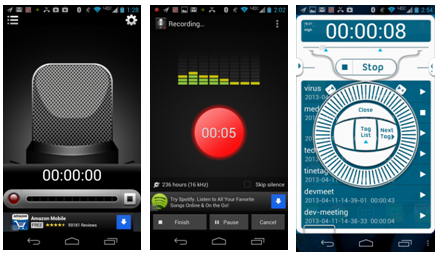
\includegraphics[width=0.7\linewidth]{./imagens1}
				\caption{ Representação gráfica das aplicações acima referidas}
				\label{fig:imagens1}
			\end{figure}
		\subsection{Tradutor de Voz para Texto}	
			\begin{itemize}
				\item ListNote Fala-para-texto Notas;
				\item Speech To Text;
				\item Text to Speech - Voice to Text; 
			\end{itemize}
			
			\begin{figure}[h]
\centering
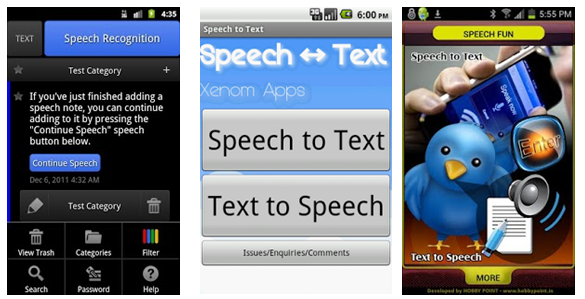
\includegraphics[width=0.7\linewidth]{./imagens2}
\caption{Representação gráfica das aplicações anteriormente referidas}
\label{fig:imagens2}
\end{figure}

\newpage

	\section{Conclusão}
	Não foi encontrada nenhuma aplicação similar ao sistema solicitado, apesar de se ter encontrado inúmeras aplicações que apenas conseguem realizar parte do projeto, designadamente na gravação de voz, e na tradução da voz para texto.
	
	
	\section{Bibliografia}	
	
	    	https://play.google.com/store/apps\\	
		
		http://www.techrepublic.com/blog/smartphones/top-four-android-voice-recorder-applications/\\
			
		http://www.tutorialspoint.com/android/androidaudiocapture.htm\\	
		
		http://developer.android.com/reference/android/media/AudioRecord.html\\	
		
		http://developer.android.com/guide/topics/media/audio-capture.html\\
	
	\section{Open Source Softwares}
	
	Mi Sound Recorder:
	http://forum.xda-developers.com/showthread.php?t=1752011\\
	
	Auphonic Software:
	http://auphonic.com/\\
	
	Rehearsal Assistant:
	http://sourceforge.net/projects/rehearsalassist/\\
	
	Android Voice Recognition Tutorial
	http://www.javacodegeeks.com/2012/08/android-voice-recognition-tutorial.html\\
	
		


		
	
\end{document}
